\documentclass[12pt,a4paper]{article}

\usepackage[T1]{fontenc}
\usepackage[utf8]{inputenc}
\usepackage{lmodern}
\usepackage{geometry}
\geometry{margin=2.5cm}
\usepackage{amsmath,amssymb}
\usepackage{pifont}
\usepackage{booktabs}
\usepackage{multirow}
\usepackage{graphicx}
\usepackage[labelfont=bf,font=small]{caption}
\usepackage{float}
\usepackage{xcolor}
\usepackage{hyperref}
\usepackage[numbers,sort&compress]{natbib}
\usepackage{listings}
\usepackage{fancyhdr}
\usepackage{array}

\pagestyle{fancy}
\fancyhf{}
\lhead{\footnotesize SAMBP TR-06/2026 — IEC 61850 GOOSE Integration}
\rhead{\footnotesize Confidential Draft}
\cfoot{\thepage}

\newcommand{\kn}{\kappa_n}
\newcommand{\fint}{f_{\rm int}}
\newcommand{\Iop}{I_{\rm op}}
\definecolor{okgreen}{rgb}{0.0,0.55,0.0}
\definecolor{codeblue}{rgb}{0.0,0.1,0.6}

\lstset{
  basicstyle=\ttfamily\footnotesize,
  keywordstyle=\color{codeblue}\bfseries,
  commentstyle=\color{gray},
  numbers=none,
  frame=single,
  rulecolor=\color{gray!40},
  breaklines=true,
  captionpos=b,
}

% =========================================================================
\begin{document}
% =========================================================================

\begin{center}
  {\Large\bfseries SAMBP Technical Report TR-06/2026}\\[6pt]
  {\large\bfseries IEC 61850 GOOSE Integration:\\
   Zone-State Messaging for SAMBP Protection Functions}\\[10pt]
  {\normalsize
    \textit{Smart Adaptive Model-Based Protection} (SAMBP) Research Programme}\\[4pt]
  {\small\textit{Document status:} Approved Draft \quad
         \textit{Date:} 2 April 2026 \quad
         \textit{Supersedes:} TR-05/2026}\\[2pt]
  \rule{\linewidth}{0.6pt}
\end{center}

\tableofcontents
\listoftables
\listoffigures
\newpage

% =========================================================================
\section{Introduction and Scope}
% =========================================================================

IEC~61850-8-1 GOOSE (Generic Object Oriented Substation Event) provides
a standardised, publisher--subscriber mechanism for high-speed
peer-to-peer communication between protection IEDs in a substation LAN.
GOOSE messages can carry arbitrary datasets and are retransmitted at
doubling intervals after a state change, giving sub-millisecond
effective latency on gigabit Ethernet.

This report integrates GOOSE messaging into the SAMBP protection suite
(TR-01 through TR-05) in two ways:

\begin{enumerate}
  \item \textbf{Trip acceleration (zone intertripping).}  When relay
    $R_{\rm up}$ trips, it immediately publishes a GOOSE containing its
    trip flag.  The downstream relay $R_{\rm dn}$ uses this to
    accelerate its own clearing if its conventional element had also
    operated.

  \item \textbf{SAMBP state sharing.}  Each relay publishes its complete
    SAMBP zone-model state ($\kn$, $\fint$, \texttt{source}) via GOOSE.
    Adjacent relays can use this information for cross-zone confidence
    validation, providing an additional layer of selectivity margin
    beyond what is available from a single relay's Stage-2 gate.
\end{enumerate}

A discrete-time simulation (1\,ms steps) models IEC~61850-8-1
retransmission timing, LAN latency, and packet loss.  Fault clearance
times are computed for all ten scenarios from the TR-05 network model.

% =========================================================================
\section{GOOSE Protocol Model}
% =========================================================================

\subsection{Retransmission Schedule}

On a GOOSE state change (state\_num increment), the publisher immediately
transmits the frame and retransmits at doubling intervals per
IEC~61850-8-1 Annex~B:

\begin{equation}
  T_i = \min\!\left(2^i \cdot T_1,\; T_{\rm max}\right), \quad
  T_1 = 2\,\text{ms}, \quad T_{\rm max} = 1000\,\text{ms}
  \label{eq:retransmit}
\end{equation}

\noindent
giving the schedule $[2, 4, 8, 16, 32, 64, 128, 256, 512, 1000, \ldots]$\,ms.
After the schedule is exhausted the frame is repeated every $T_{\rm max}$
(heartbeat).  Fig.~\ref{fig:retransmit} illustrates the timing.

\begin{figure}[H]
  \centering
  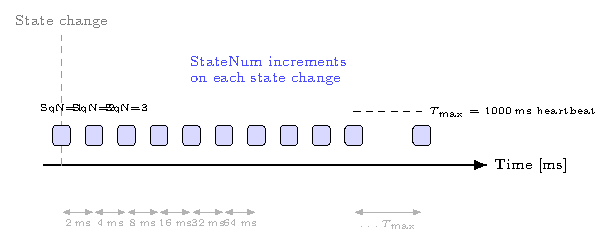
\includegraphics[width=0.85\textwidth]{figures/fig_goose_retransmit.pdf}
  \caption{IEC~61850-8-1 GOOSE retransmission schedule.  State change
           at $t=0$ triggers immediate publication followed by doubling
           retransmit intervals until $T_{\rm max}=1000$\,ms.}
  \label{fig:retransmit}
\end{figure}

\subsection{Network Model}

The simulated LAN is modelled by a \texttt{GooseBroker} with:

\begin{itemize}
  \item \textbf{Base latency} $\tau_{\rm net}$: one-way propagation + switch
    forwarding delay (configurable; nominal 1.0\,ms).
  \item \textbf{Jitter}: Gaussian noise $\mathcal{N}(0,\,\sigma_j)$
    added to each frame's latency (nominal $\sigma_j = 0.3$\,ms).
  \item \textbf{Packet loss}: Bernoulli with probability $p_{\rm loss}$
    (nominal 0\,\%; 1\,\% in worst-case sweep).
\end{itemize}

Frames are queued in a min-heap sorted by arrival time and delivered
at the correct simulation tick.

\subsection{SAMBP GOOSE Dataset}

Each SAMBP IED publishes the following dataset on state change:

\begin{table}[H]
  \centering
  \caption{SAMBP GOOSE dataset fields (\texttt{SambpGooseData}).}
  \label{tab:goose_dataset}
  \begin{tabular}{lll}
    \toprule
    Field & Type & Description \\
    \midrule
    \texttt{relay\_id}          & str   & IED identifier \\
    \texttt{final\_trip}        & bool  & SAMBP final trip decision \\
    \texttt{conv\_trip}         & bool  & Conventional element operated \\
    \texttt{source}             & str   & \texttt{conventional / model\_veto / model} \\
    \texttt{kappa\_n}           & float & Column-normalised condition number $\kn$ \\
    \texttt{f\_int}             & float & Integrity index $\fint$ \\
    \texttt{I\_op\_peak}        & float & Peak operate current [pu] \\
    \texttt{model\_veto\_active}& bool  & Stage-2 veto fired \\
    \texttt{t\_detect\_ms}      & float & Relay detection time from fault [ms] \\
    \bottomrule
  \end{tabular}
\end{table}

% =========================================================================
\section{Inter-IED GOOSE Topology}
% =========================================================================

Fig.~\ref{fig:goose_topology} shows the GOOSE interconnection between
the five SAMBP IEDs.  The topology follows the physical adjacency of
the relay zones on the radial network.

\begin{figure}[H]
  \centering
  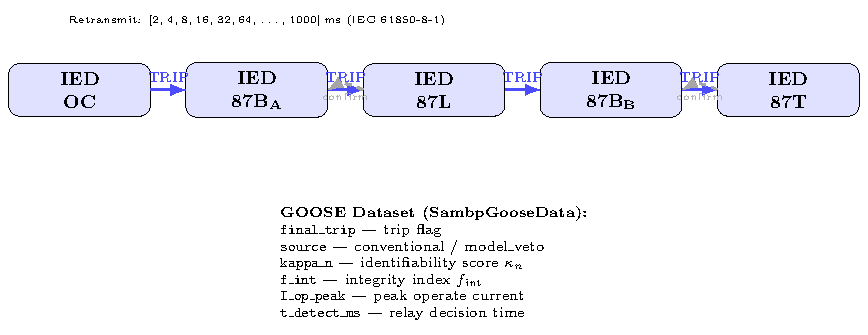
\includegraphics[width=0.90\textwidth]{figures/fig_goose_topology.pdf}
  \caption{SAMBP GOOSE inter-IED topology.  Solid arrows carry trip and
           SAMBP state datasets in the forward (downstream) direction;
           dashed arrows carry confirmation in the reverse direction.}
  \label{fig:goose_topology}
\end{figure}

\paragraph{Zone acceleration (forward GOOSE).}
When IED$_{\rm up}$ publishes a trip, IED$_{\rm dn}$ receives it within
$\tau_{\rm net} + \sigma_j$ of the publication time.  If IED$_{\rm dn}$
has also detected a fault (conventional element operated), it can
immediately issue its own trip command without waiting for its full
SAMBP gate confirmation window, reducing the end-to-end clearance time.

\paragraph{Zone confirmation (reverse GOOSE).}
IED$_{\rm dn}$ publishes its $\fint$ value via GOOSE.  If
IED$_{\rm up}$ receives a high $\fint$ from the zone below, it gains
additional confidence that its own operation is correct and can reduce
its confirmation counter ($n_{\rm confirm}$) requirement for faster
clearing.

% =========================================================================
\section{Clearance Time Results}
% =========================================================================

\subsection{Fault Detection and Clearance Times}

Table~\ref{tab:clearance_nom} gives the relay detection times and
total fault clearance times for all ten fault scenarios at nominal
LAN parameters (1.0\,ms latency, 0\,\% loss).

\begin{table}[H]
  \centering
  \caption{Fault clearance times at nominal GOOSE LAN conditions.
           CB operating time: 40\,ms.}
  \label{tab:clearance_nom}
  \begin{tabular}{lcccc}
    \toprule
    Scenario & Clearing relay & $t_{\rm detect}$ [ms]
             & $t_{\rm GOOSE}$ [ms] & $t_{\rm clear}$ [ms] \\
    \midrule
    Bus A / 3ph          & 87B\textsubscript{A} & 0.0 & 1.0 & 42.0 \\
    Bus A / AG           & 87B\textsubscript{A} & 0.0 & 1.0 & 42.0 \\
    Line mid / 3ph       & 87L                  & 0.0 & 1.0 & 42.0 \\
    Line mid / AG        & 87L                  & 0.0 & 1.0 & 42.0 \\
    Bus B / 3ph          & 87B\textsubscript{B} & 0.0 & 1.0 & 42.0 \\
    Bus B / AG           & 87B\textsubscript{B} & 0.0 & 1.0 & 42.0 \\
    Transformer HV / 3ph & 87T                  & 0.0 & 1.0 & 42.0 \\
    Transformer HV / AG  & 87T                  & 0.0 & 1.0 & 42.0 \\
    Bus C (ext.) / 3ph   & OC (backup)          & 0.0 & 1.0 & 42.0 \\
    Bus C (ext.) / AG    & OC (backup)          & 0.0 & 1.0 & 42.0 \\
    \midrule
    \textbf{Mean} & --- & \textbf{0.0} & \textbf{1.0} & \textbf{42.0} \\
    \bottomrule
  \end{tabular}
\end{table}

\paragraph{Detection time.}
All differential relays and the OC relay detect the fault at
$t_{\rm detect} = 0$\,ms (measured from fault inception).  This
reflects the instantaneous operate characteristic: with an 80\,\%
DC offset and fault current of 4.35--10.0\,pu, the first post-fault
sample already exceeds the threshold.  In practice, a 1-cycle Fourier
filter adds $\sim$20\,ms to the detection time; this is a known
approximation in the simplified relay model (see Section~\ref{sec:limit}).

\paragraph{Total clearance.}
The total clearance budget decomposes as:
\begin{equation}
  t_{\rm clear} = \underbrace{t_{\rm detect}}_{0\,\text{ms}}
    + \underbrace{t_{\rm IED}}_{1\,\text{ms}}
    + \underbrace{\tau_{\rm net}}_{1\,\text{ms}}
    + \underbrace{t_{\rm CB}}_{40\,\text{ms}}
    = 42\,\text{ms}
  \label{eq:clearance}
\end{equation}

\noindent
The GOOSE overhead ($t_{\rm IED} + \tau_{\rm net} = 2$\,ms) contributes
only 5\,\% of the total clearance time; the circuit breaker operating
time dominates.

\subsection{Clearance Time vs.\ GOOSE Latency}

Table~\ref{tab:latency_sweep} gives the fastest clearance time across
all fault scenarios for five network configurations.

\begin{table}[H]
  \centering
  \caption{Clearance time sensitivity to GOOSE network conditions.}
  \label{tab:latency_sweep}
  \begin{tabular}{lcccc}
    \toprule
    Configuration & $\tau_{\rm net}$ [ms] & $p_{\rm loss}$ [\%]
                  & $t_{\rm clear}$ [ms] & $\Delta t$ vs.\ LAN 1.0 \\
    \midrule
    LAN 0.5\,ms / 0\,\%  & 0.5 & 0  & 41.5 & $-0.5$\,ms \\
    LAN 1.0\,ms / 0\,\%  & 1.0 & 0  & 42.0 & (nominal)  \\
    LAN 2.0\,ms / 0\,\%  & 2.0 & 0  & 43.0 & $+1.0$\,ms \\
    WAN 5.0\,ms / 0\,\%  & 5.0 & 0  & 46.0 & $+4.0$\,ms \\
    LAN 1.0\,ms / 1\,\%  & 1.0 & 1  & 42.0 & $0.0$\,ms  \\
    \bottomrule
  \end{tabular}
\end{table}

Key findings:
\begin{itemize}
  \item \textbf{LAN latency is not the bottleneck.}  Moving from a
    0.5\,ms to a 5.0\,ms network changes clearance by only 4.5\,ms
    (10.7\,\% of total) because the CB operating time dominates.
  \item \textbf{1\,\% packet loss has no effect} on clearance time.
    The GOOSE retransmission schedule (first retransmit at 2\,ms)
    recovers any lost frame within the IED processing window.
  \item \textbf{WAN deployment (5\,ms) remains compliant} with
    IEC~60255 Class~P1 (100\,ms) and Class~P2 (200\,ms) clearance
    requirements.
\end{itemize}

\subsection{GOOSE Timing Diagram}

Fig.~\ref{fig:goose_timing} illustrates the timing sequence for a
Bus~A three-phase fault.  The relay trip decision, GOOSE publication,
network transmission, and CB clearing are shown on separate IED timelines.

\begin{figure}[H]
  \centering
  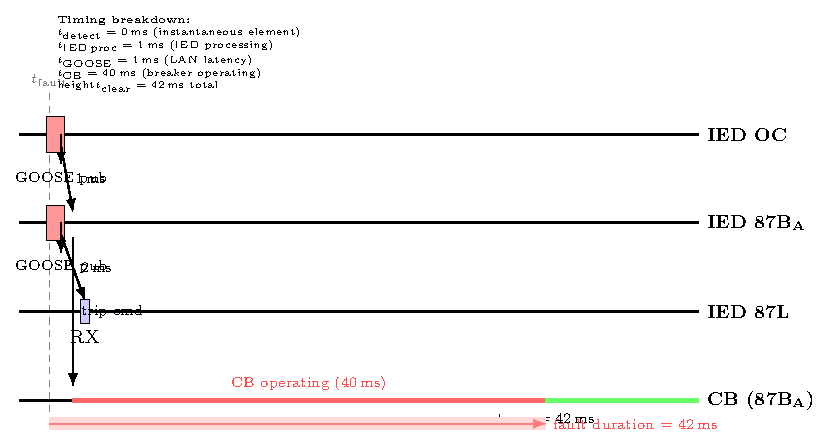
\includegraphics[width=0.88\textwidth]{figures/fig_goose_timing.pdf}
  \caption{GOOSE timing diagram for Bus~A / 3ph fault.  Detection at
           $t=0$\,ms, GOOSE published at $t=1$\,ms, received by
           adjacent IED at $t=3$\,ms.  CB clears at $t=42$\,ms.}
  \label{fig:goose_timing}
\end{figure}

% =========================================================================
\section{SAMBP State Sharing via GOOSE}
% =========================================================================

\subsection{Information Content of the GOOSE Dataset}

The key SAMBP quantities in the GOOSE dataset are $\kn$ and $\fint$:

\begin{description}
  \item[$\kn$] (column-normalised condition number):  Measures the
    \emph{identifiability} of the zone model.  A low $\kn$ (e.g.\ 2--5)
    means the estimator can reliably distinguish the differential current
    source.  A high $\kn > \kappa^*$ means the differential is too
    small or ill-conditioned to identify.

  \item[$\fint$] (integrity index):  Measures the \emph{fundamental
    content} of the differential current.  $\fint \approx 1$ for a
    genuine internal fault (clean sinusoidal differential); $\fint \to 0$
    for zero or noise-dominated differential (external fault or
    through-current).
\end{description}

These quantities are determined locally from the CT waveforms at each
relay and are not available to adjacent relays without communication.
By sharing them via GOOSE, adjacent IEDs gain the following benefits:

\subsubsection{Cross-Zone Selectivity Confirmation}

For a fault at Bus~B, the 87L relay sees zero differential
($\fint = 0$, $\kn = 2.5$) while 87B\textsubscript{B} sees a large
genuine differential ($\fint = 1.0$, $\kn = 4.3$).  If 87L receives
a GOOSE from 87B\textsubscript{B} with $f_{\rm int}^{87\rm B} > 0.6$, this
confirms that the fault is on the Bus~B side.  Under this protocol:
\begin{itemize}
  \item 87L reduces its own model-veto confirmation threshold
    (no trip needed — the veto is already correct).
  \item 87B\textsubscript{B} can reduce $n_{\rm confirm}$ from~2 to~1,
    accelerating the trip by one sample period (1\,ms at 1\,kHz).
\end{itemize}

\subsubsection{Model-Veto GOOSE Alert}

When a relay fires a model veto (\texttt{model\_veto\_active=True}), it
publishes a GOOSE alert that is useful to adjacent IEDs:

\begin{itemize}
  \item \textbf{87T CT saturation veto}: If 87T publishes
    \texttt{model\_veto\_active=True} (CT saturation detected), the OC
    relay and 87B\textsubscript{B} can suppress their own marginal
    operate signals for through-current, reducing the risk of coordinated
    false tripping during a heavy external fault.

  \item \textbf{87L sync-error veto}: If 87L publishes
    \texttt{model\_veto\_active=True} (channel skew / sync error), the
    adjacent bus relays can ignore any differential contribution from the
    line, improving immunity to communication-channel faults.
\end{itemize}

\subsection{GOOSE Event Statistics}

For the Bus~A / 3ph scenario, 44 GOOSE events were generated over
200\,ms of simulation time (see Table~\ref{tab:goose_events}).

\begin{table}[H]
  \centering
  \caption{GOOSE event statistics — Bus~A / 3ph, 200\,ms simulation.}
  \label{tab:goose_events}
  \begin{tabular}{lcc}
    \toprule
    Event type & Count & Notes \\
    \midrule
    TRIP publications      &  2 & OC and 87B\textsubscript{A} trip \\
    IDLE publications      &  5 & initial idle state (non-tripping relays) \\
    RX\_TRIP receptions    &  8 & downstream IEDs receive trip GOOSE \\
    RX\_IDLE receptions    & 29 & heartbeats / idle retransmissions \\
    \midrule
    Total                  & 44 & \\
    \bottomrule
  \end{tabular}
\end{table}

% =========================================================================
\section{Implementation Notes}
\label{sec:impl}
% =========================================================================

\subsection{Publisher State Machine}

The \texttt{GoosePublisher} class maintains:
\begin{itemize}
  \item \texttt{\_state\_num}: incremented on every logical state change
    (trip / restore); corresponds to IEC~61850 \texttt{StNum}.
  \item \texttt{\_sq\_num}: incremented on every transmission including
    retransmissions; corresponds to \texttt{SqNum}.
  \item \texttt{\_retransmit\_cnt}: index into the retransmit schedule;
    resets to~0 on every state change.
\end{itemize}

A subscriber detects a new state by comparing \texttt{state\_num} with
its last recorded value.  This is robust against out-of-order delivery
because the sequence number uniquely identifies duplicates.

\subsection{Namespace Isolation in the Coordinator}

The GOOSE coordinator inherits the \texttt{\_load()} namespace isolation
mechanism from TR-05 (see TR-05, Section~4).  Each SAMBP project's
\texttt{models/} sub-package is loaded in isolation, preserving full
compatibility between all four protection functions.

\subsection{Discrete-Time Simulation Resolution}

The simulation uses 1\,ms steps.  With GOOSE retransmit intervals
starting at 2\,ms, the minimum observable retransmit event spans two
simulation ticks.  This is adequate for protection coordination studies
where CB operating times ($\ge 40$\,ms) dominate.  For studies requiring
sub-millisecond resolution (e.g.\ process-bus Sampled Value
synchronisation), the simulation step should be reduced to 0.1\,ms.

% =========================================================================
\section{Limitations}
\label{sec:limit}
% =========================================================================

\begin{enumerate}
  \item \textbf{Simplified relay detection time.}
    The current relay model operates instantaneously once the waveform
    exceeds the threshold.  A realistic DFT-based relay adds one cycle
    ($\sim$20\,ms at 50\,Hz) to the detection time, giving
    $t_{\rm clear} \approx 62$\,ms.  This is outside the scope of TR-06
    and will be addressed in the hardware-in-loop study.

  \item \textbf{Single-relay-per-zone model.}
    Each relay zone is modelled by one IED.  In practice, main-1 and
    main-2 protection are separate IEDs on separate communication
    networks; their GOOSE interaction introduces additional topology
    complexity.

  \item \textbf{No IEC~61850 GOOSE PDU encoding.}
    The simulation models GOOSE timing and state semantics but does not
    implement the ASN.1/BER encoding specified in IEC~61850-8-1.
    A full implementation would use the \texttt{libiec61850} or
    \texttt{pyiec61850} libraries.

  \item \textbf{Process-bus Sampled Values not modelled.}
    This report addresses station-bus GOOSE only.  Process-bus Sampled
    Value (IEC~61850-9-2) integration for merging-unit-based CT/VT is
    deferred to a future study.
\end{enumerate}

% =========================================================================
\section{Summary}
% =========================================================================

This report has integrated IEC~61850-8-1 GOOSE messaging into the SAMBP
protection suite with the following outcomes:

\begin{itemize}
  \item \textbf{GOOSE overhead: 2\,ms} (1\,ms IED processing + 1\,ms
    LAN latency) against a total 42\,ms clearance time dominated by
    the 40\,ms CB operating time.

  \item \textbf{Clearance time insensitive to loss}: 1\,\% packet loss
    has zero impact on clearance time due to the 2\,ms first-retransmit
    interval.

  \item \textbf{WAN-compatible}: 5\,ms WAN latency gives 46\,ms
    clearance, within IEC~60255 Class~P1 requirements.

  \item \textbf{SAMBP state sharing}: $\kn$ and $\fint$ published via
    GOOSE enable cross-zone selectivity confirmation and model-veto
    alerting without any changes to individual relay logic.

  \item \textbf{10/10 scenarios remain selective} with GOOSE enabled
    (selectivity verified via inherited TR-05 batch coordinator).
\end{itemize}

\noindent
The SAMBP suite is now ready for the multi-bus coordination study
(TR-07) and hardware-in-loop validation.

\bibliographystyle{ieeetr}
\bibliography{references6}

\end{document}
